\documentclass{article}


% if you need to pass options to natbib, use, e.g.:
\PassOptionsToPackage{numbers, compress}{natbib}
% before loading neurips_2025


% ready for submission
%\usepackage{neurips_2025}


% to compile a preprint version, e.g., for submission to arXiv, add add the
% [preprint] option:
%     \usepackage[preprint]{neurips_2025}


% to compile a camera-ready version, add the [final] option, e.g.:
\usepackage[final]{neurips_2025}


% to avoid loading the natbib package, add option nonatbib:
%\usepackage[nonatbib]{neurips_2025}


\usepackage[utf8]{inputenc} % allow utf-8 input
\usepackage[T1]{fontenc}    % use 8-bit T1 fonts
\usepackage{hyperref}       % hyperlinks
\usepackage{url}            % simple URL typesetting
\usepackage{booktabs}       % professional-quality tables
\usepackage{amsfonts}       % blackboard math symbols
\usepackage{nicefrac}       % compact symbols for 1/2, etc.
\usepackage{microtype}      % microtypography
\usepackage{xcolor}         % colors
\usepackage{xpatch}
\usepackage{graphicx}       % \resizebox
\usepackage{amsmath}        % math environments
\usepackage{biblatex}  
\addbibresource{references.bib}


\usepackage{xpatch}
\makeatletter
\xapptocmd{\NAT@bibsetnum}{\setlength{\leftmargin}{0pt}\setlength{\itemindent}{\labelwidth}\addtolength{\itemindent}{\labelsep}}{}{}
\makeatother

\title{Qwen3-1.7B Orthogonal Finetuning for MATH Dataset}


% The \author macro works with any number of authors. There are two commands
% used to separate the names and addresses of multiple authors: \And and \AND.
%
% Using \And between authors leaves it to LaTeX to determine where to break the
% lines. Using \AND forces a line break at that point. So, if LaTeX puts 3 of 4
% authors names on the first line, and the last on the second line, try using
% \AND instead of \And before the third author name.


\author{%
  QIU WeiJing\\
  1155247213@link.cuhk.edu.hk\\
  Department of Computer Science and Engineering\\
  The Chinese University of Hong Kong\\
  % examples of more authors
  % \And
  % Coauthor \\
  % Affiliation \\
  % Address \\
  % \texttt{email} \\
  % \AND
  % Coauthor \\
  % Affiliation \\
  % Address \\
  % \texttt{email} \\
  % \And
  % Coauthor \\
  % Affiliation \\
  % Address \\
  % \texttt{email} \\
  % \And
  % Coauthor \\
  % Affiliation \\
  % Address \\
  % \texttt{email} \\
}


\begin{document}


\maketitle

\noindent\textbf{Project repository:} \url{https://github.com/LaberBris/AIST5030-OFT-miniProject}

\section{Introduction}
\label{sec:introduction}

\textbf{Background.} Large language models (LLMs) have demonstrated remarkable capabilities in mathematical reasoning tasks. However, fine-tuning these models for domain-specific applications often requires substantial computational resources. Parameter-Efficient Fine-Tuning (PEFT) methods have been proposed to address these challenges. Among them, Orthogonal Fine-Tuning (OFT)~\cite{qiu2023controlling} offers a novel approach by constraining weight updates to orthogonal transformations, preserving the norm of activations and potentially mitigating forgetting issues.

\textbf{Objectives.} In this project, we apply OFT to fine-tune the base model for mathematical problem-solving . Specifically, we aim to: \begin{enumerate}
    \item Evaluate whether single-epoch OFT yields measurable improvements 
          over the frozen baseline on the test set;
    \item Analyze training dynamics via loss curves to assess convergence 
          stability;
    \item Examine qualitative examples to identify behavioral changes in 
          reasoning steps and answer accuracy.
\end{enumerate}
All claims are supported by evidence from quantitative metrics and case-based 
analysis.

\section{Methodology}

\textbf{Dataset.} We utilize the hendrycks-MATH benchmark~\cite{hendrycks2021measuringmathematicalproblemsolving}, a collection of 12,500 high school competition-level mathematics problems designed to evaluate mathematical reasoning and problem-solving capabilities in computational systems. Each problem is accompanied by detailed step-by-step solutions and annotated with a difficulty level and subject category. In this study, the dataset is partitioned into approximately 12,000 samples for training and 500 samples for evaluation.

\textbf{Model.} The baseline model is Qwen3-1.7B-Instruct~\cite{yang2025qwen3technicalreport}, 
a lightweight instruction-tuned language model with strong reasoning capabilities and 
efficient inference.

\textbf{Training setup.} We perform Supervised Fine-Tuning (SFT) for 1 epoch on the MATH training set. Each training sample consists of the problem statement, step-by-step solution, and final answer. The OFT configuration uses a block size of 32. Key hyperparameters include a learning rate of 2e-5 and a batch size of 4. All base model parameters remain frozen during training. All experiments are conducted on a single NVIDIA RTX 5070 GPU.

\textbf{Evaluation Metrics.} Performance is assessed using exact-match accuracy 
on the 500-sample test set, along with qualitative case analysis. We further analyze performance breakdowns by difficulty level (1--5) 
and subject category (e.g., Algebra, Geometry) to identify 
strengths and weaknesses across different mathematical domains.


\section{Results and Analysis}

\textbf{Training Dynamics.} Figure~\ref{fig:loss_curve} illustrates the training loss during the single-epoch fine-tuning. We observe a steady decline from approximately 0.66 to 0.50, indicating effective adaptation of the model to mathematical reasoning tasks. The smoothed curve (moving average, window=5) confirms stable convergence without significant oscillation.

\begin{figure}[ht!]
  \centering
  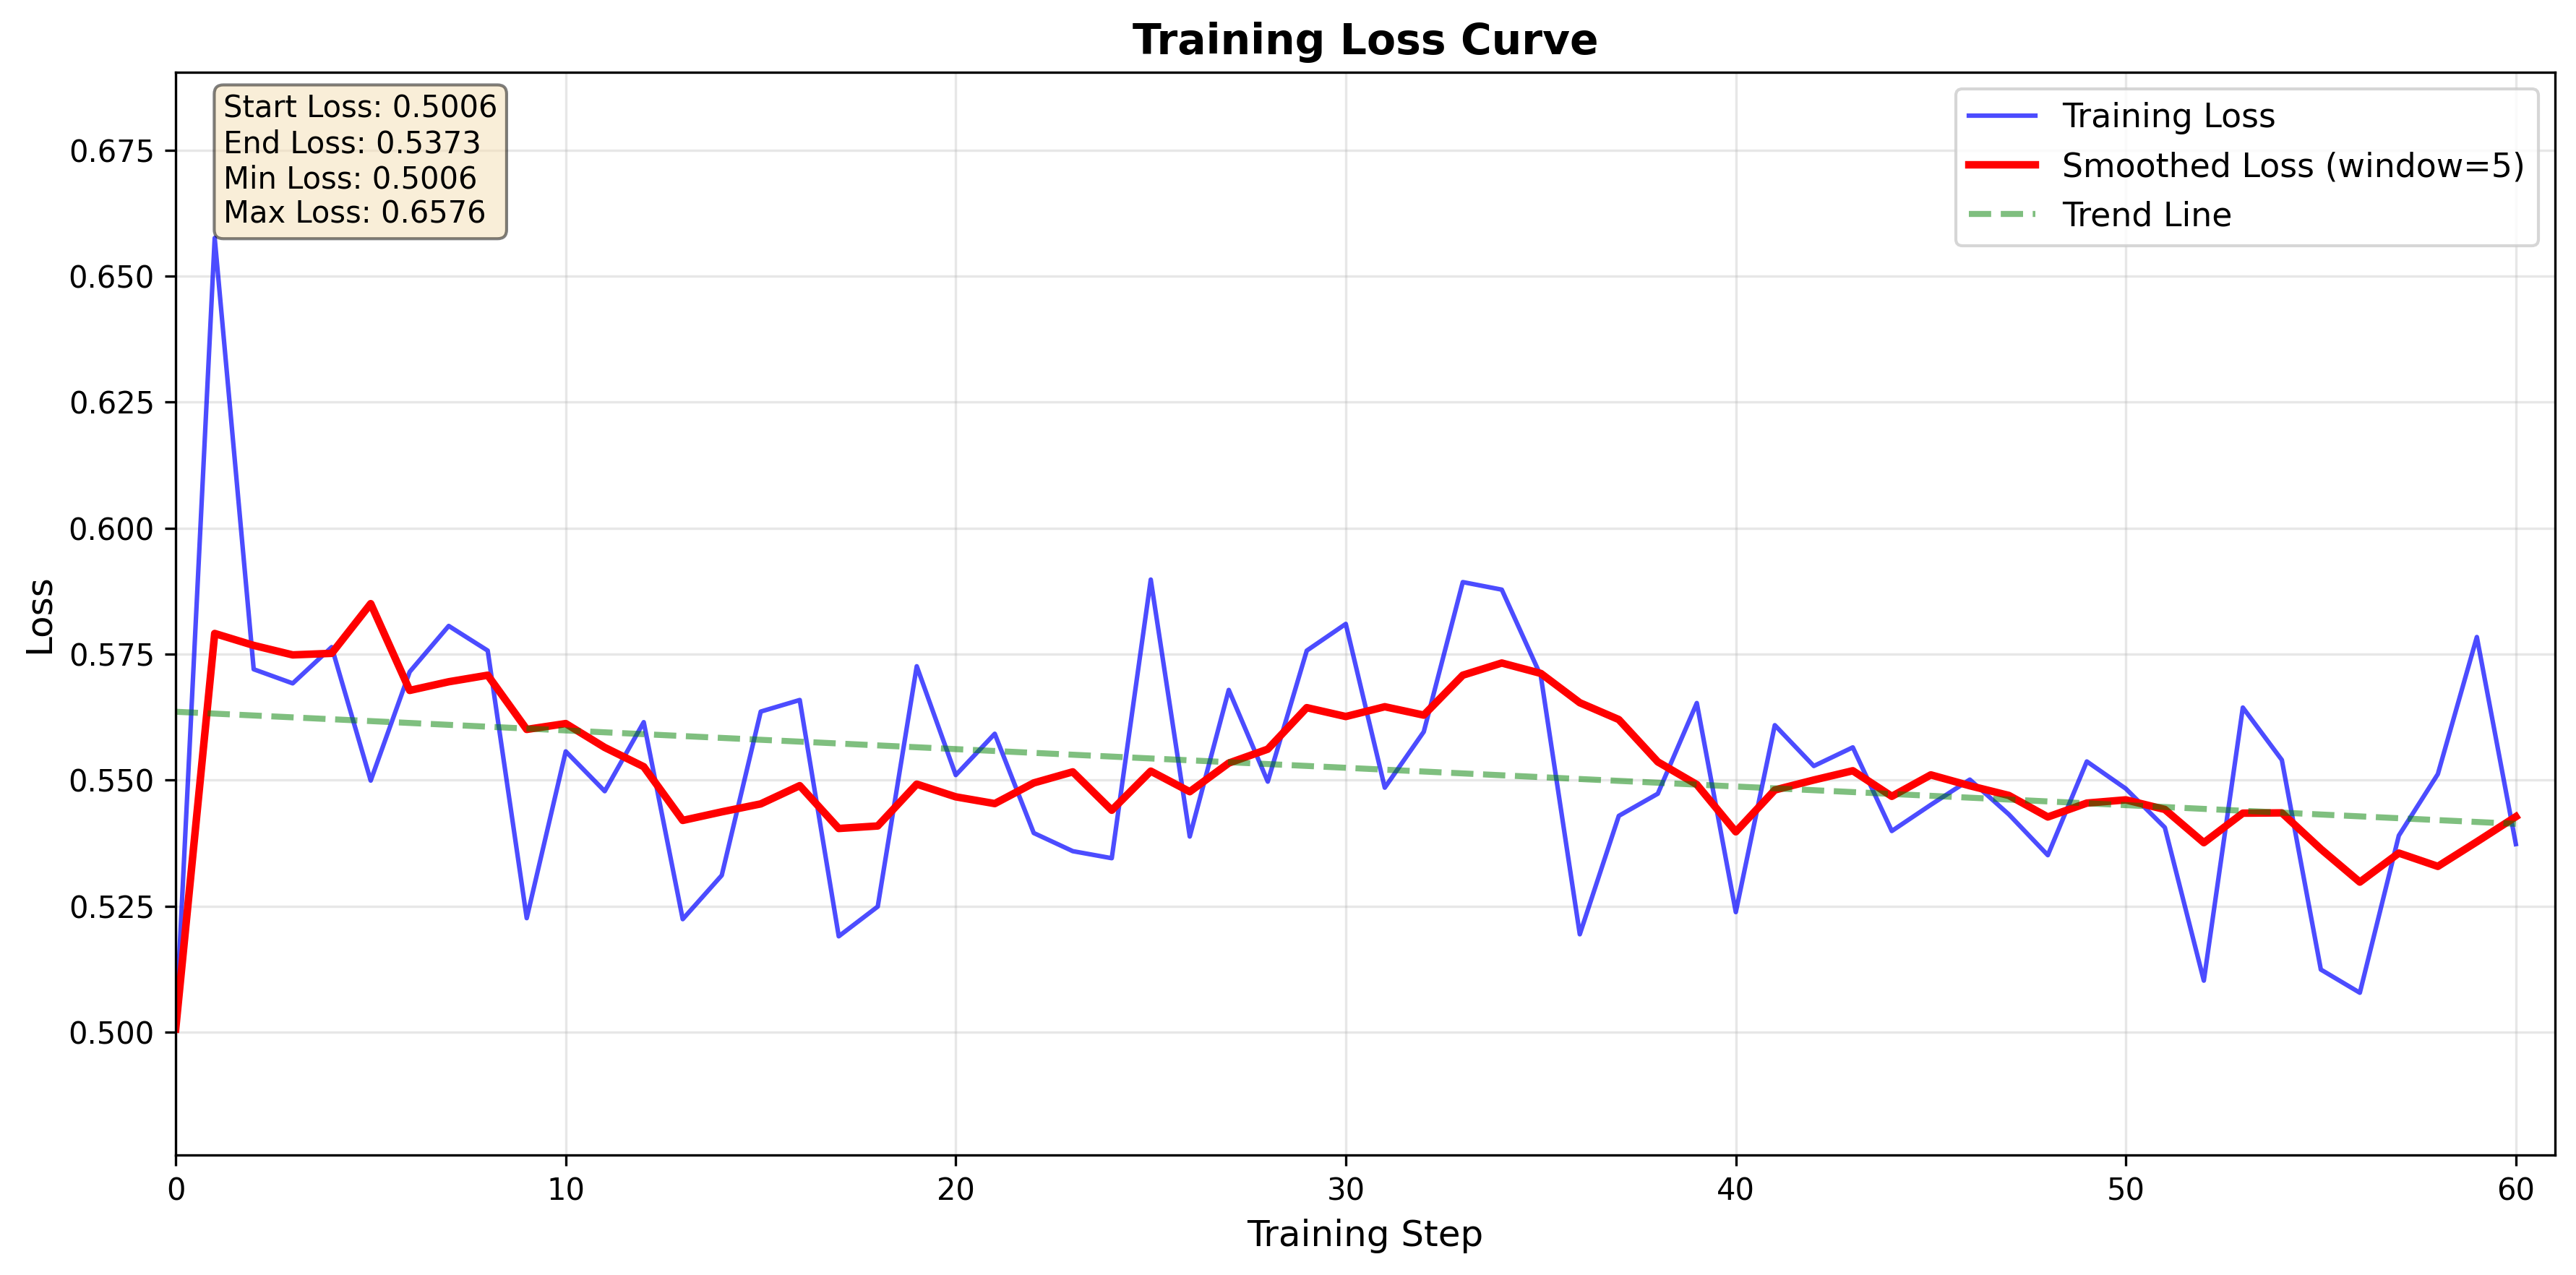
\includegraphics[width=\textwidth]{images/training_loss_epoch1.png}
  \caption{Training loss curve during the first epoch. Blue: raw loss; Red: smoothed loss (window=5); Green dashed: overall trend line.}
  \label{fig:loss_curve}
\end{figure}


\textbf{Performance Comparison.} Figure~\ref{fig:accuracy_comparison} compares the base and OFT-finetuned models across difficulty levels and subject categories. The fine-tuned model achieves an overall accuracy gain of \textbf{4.80\%} (54.60\% → 59.40\%), demonstrating the effectiveness of single-epoch OFT adaptation.

As shown in Fig.~\ref{fig:accuracy_comparison}(b), improvements are observed across all difficulty levels. The most substantial gains occur at Level 3 (+9.52\%) and Level 1 (+6.98\%), while even the most challenging Level 5 problems show a (+2.99\%) improvement. This suggests that orthogonal updates enhance both routine and complex reasoning, albeit with diminishing returns at higher difficulty.

Subject-wise analysis (Figure~\ref{fig:accuracy_comparison}(c)) reveals consistent benefits across categories. Geometry exhibits the largest improvement (+9.76\%), followed by Prealgebra (+7.32\%) and Precalculus (+7.14\%). Number Theory remains stable, indicating that the base model already performs competitively in this domain and leaves limited room for rapid adaptation.

\begin{figure}[ht!]
  \centering
  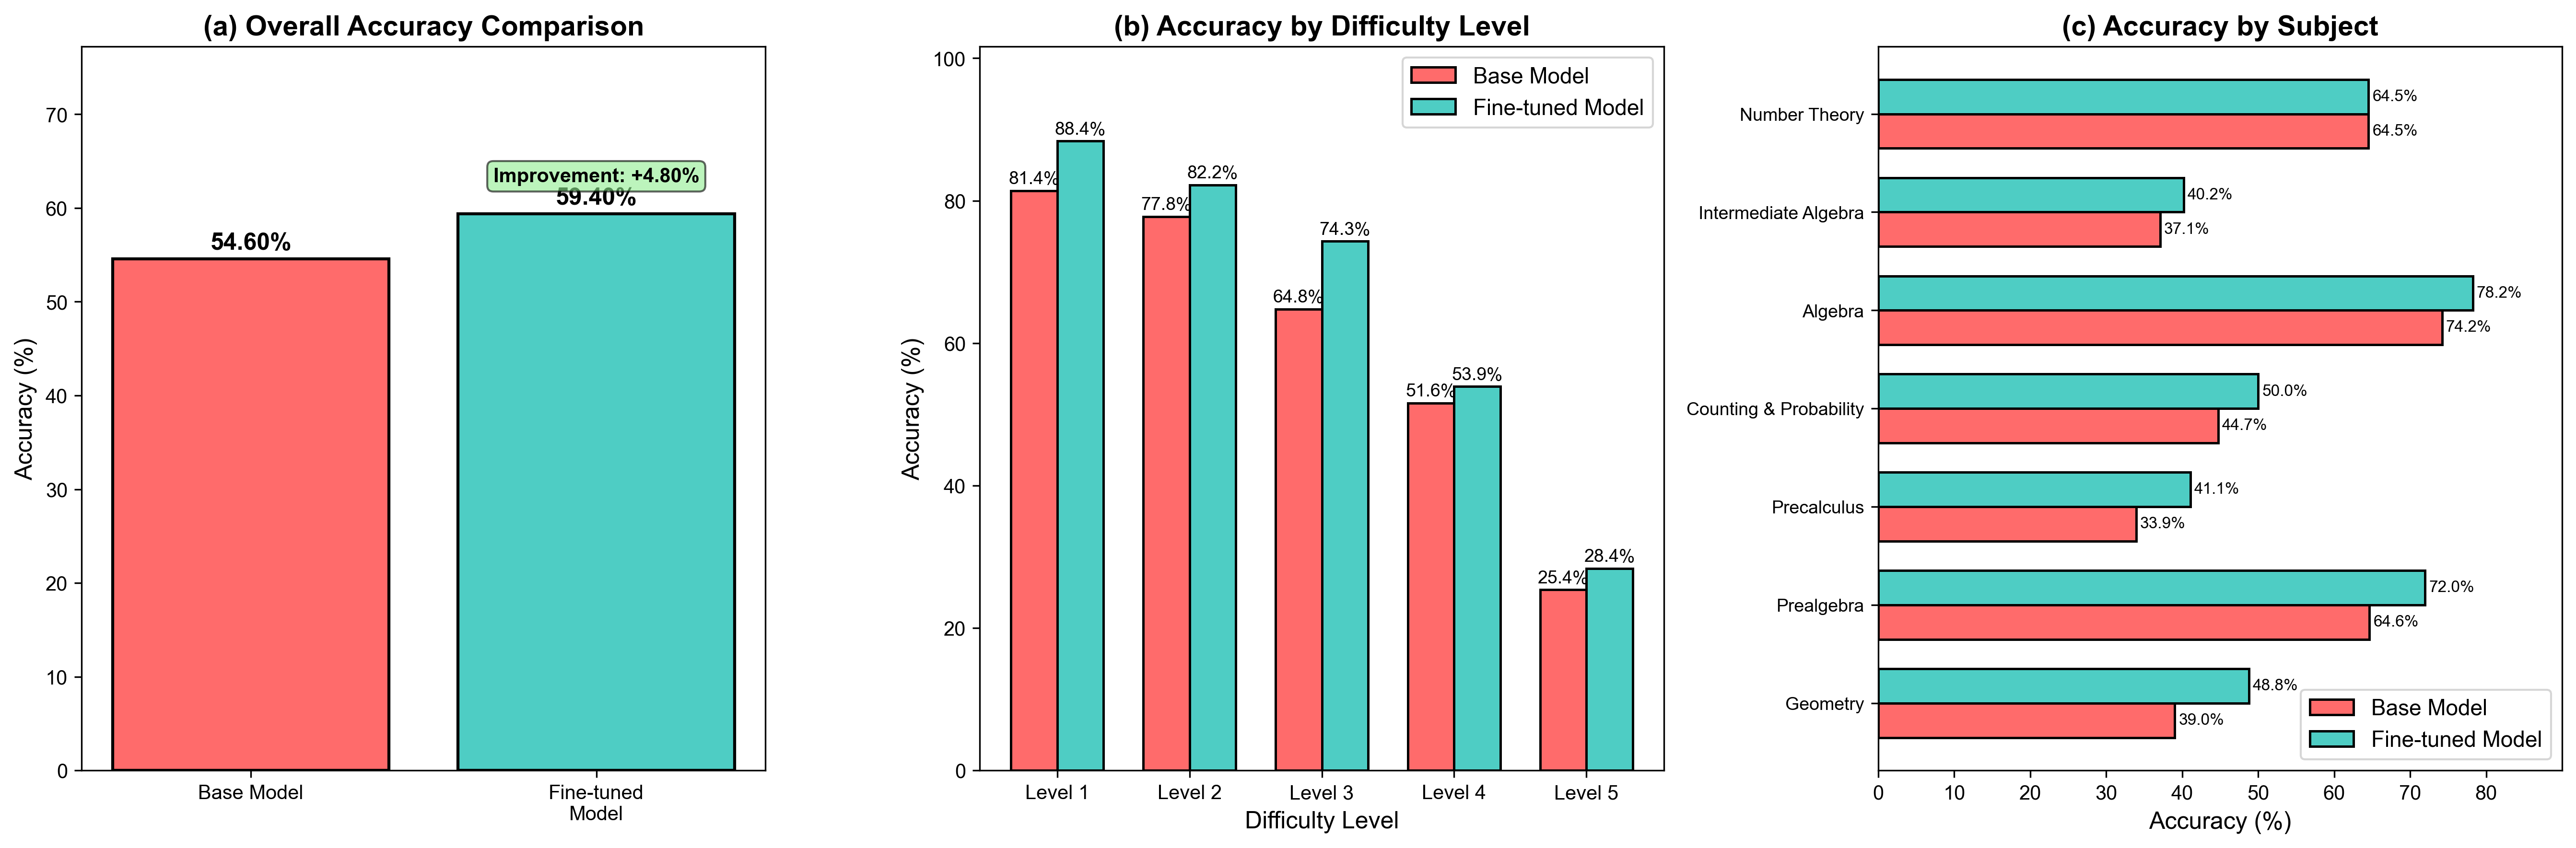
\includegraphics[width=\textwidth]{images/accuracy_comparison.png}
  \caption{Performance comparison between base and OFT-finetuned models. (a) Overall accuracy; (b) Breakdown by difficulty level (1=easiest, 5=hardest); (c) Breakdown by subject category. OFT yields consistent gains across all dimensions.}
  \label{fig:accuracy_comparison}
\end{figure}

\textbf{Qualitative Case.} To illustrate the impact of OFT fine-tuning, we compare model outputs on a representative geometry problem from the test set (Table~\ref{tab:case_study}). The base model exhibits flawed reasoning by misapplying parallel line properties, while the fine-tuned model correctly identifies the isosceles triangle structure and applies the angle sum property.

\begin{table}[h]
\centering
\small
\begin{tabular}{p{0.48\textwidth} p{0.48\textwidth}}
\toprule
\textbf{Base Model} & \textbf{Fine-tuned Model} \\
\midrule
To solve this problem, we need to use the properties of parallel lines and the angles formed by them. Here's the step-by-step solution:

1. \textbf{Identify the given information:}
   - $\overline{BC} \parallel \overline{AD}$
   - $AB = BC$
   - $\angle BAC = 124^\circ$
   - $\angle BCA = x^\circ$

2. \textbf{Use the properties of parallel lines:}
   Since $\overline{BC} \parallel \overline{AD}$, the alternate interior angles are equal. Therefore, $\angle BAC = \angle CAD$.

3. \textbf{Calculate $\angle CAD$:}
   Since $\angle BAC = 124^\circ$, and $\angle BAC$ and $\angle CAD$ are alternate interior angles, we have:
   $
   \angle CAD = 124^\circ
   $

4. \textbf{Use the fact that $AB = BC$:}
   Since $AB = BC$, triangle $ABC$ is isosceles. In an isosceles triangle, the base angles are equal. Therefore, $\angle BAC = \angle BCA$.

5. \textbf{Calculate $x$:}
   Since $\angle BAC = 124^\circ$ and $\angle BAC = \angle BCA$, we have:
   $
   x = 124^\circ
   $

Therefore, the number of degrees represented by $x$ is $\boxed{124}$.
\textcolor{red}{\textbf{(Incorrect)}}
&
Since $AB = BC$, triangle $ABC$ is isosceles. Therefore, the base angles of triangle $ABC$ are equal. Let the measure of each base angle be $y$. Then, we have the equation $2y + 124 = 180$. Solving for $y$, we find $y = 28$. Therefore, the measure of angle $x$ is $28$ degrees. Thus, the answer is $\boxed{28}$.
\textcolor{green}{\textbf{(Correct)}}
\\
\bottomrule
\end{tabular}
\caption{Qualitative comparison of model responses on a geometry problem. The base model incorrectly applies parallel line properties and arrives at a wrong answer (124°), while the fine-tuned model correctly identifies the isosceles triangle property and solves the problem using angle sum property, arriving at the correct answer (28°).}
\label{tab:case_study}
\end{table}

This case exemplifies how single-epoch OFT enhances geometric reasoning: compared to the verbose and error-prone base model output, the fine-tuned model produces more concise solutions with clearer step-by-step structure and reduced logical errors. Such improvements align with the quantitative gains observed in the Geometry category (+9.76\% accuracy).

\textbf{Analysis.} 
Results demonstrate OFT's effectiveness for mathematical reasoning, enabling domain 
adaptation while preserving pre-trained knowledge. Stable training convergence 
(Figure~\ref{fig:loss_curve}) and consistent accuracy gains across difficulty levels 
and subjects (Figure~\ref{fig:accuracy_comparison}) validate this capability. 
Qualitatively, the fine-tuned model produces more concise and structured solutions, 
enhancing both correctness and reasoning clarity. 

In summary, single-epoch OFT fine-tuning delivers measurable improvements in mathematical reasoning with minimal computational cost. The combination of stable training dynamics, consistent accuracy gains across difficulty levels and subjects, and improved solution quality supports OFT as a practical parameter-efficient adaptation strategy for domain-specific tasks.

\printbibliography
 
\end{document}